\chapter{Project execution}

\section{Team}
This team consists of five members:

\begin{itemize}
	\item Michal Bali,
	\item Marcel Hruška,
	\item Peter Polák,
	\item Adam Šmelko,
	\item Lucia Tódová.
\end{itemize}

Each team member is responsible for delivering work packages assigned to him or her (see \cref{timeline}). 

\section{Team management} 

For managing the project and team members we use a visual process management system Kanban. Additionally, the project is developed within the environment of Broadcom Inc., which supplies additional project management and supervision. We are attempting to follow the Agile software development guidelines --- our team meets every week with our Broadcom supervisor at stand-ups and discusses the current status of particular tasks with their assignees, reviews progress and plans work for the next week. 

Slack is used for dynamic communication between team members.

\section{Project timeline}
\label{timeline}
The project was split into several milestones and work packages. Presently the milestone \hyperref[milestone_preview]{Preview} has already been reached. Therefore, there is currently a working prototype, and some of the presented work packages are already finished. 

The implementation of the whole project was planned to be accomplished within nine months. The project has been already worked on for four months which has already resulted in completion of milestone M4 Preview. Since most of the architecture, design and planning questions have been answered during the development of the prototype, we do not expect any additional technical or architectural issues at this point. Additionally, the company support from Broadcom Inc. prevents financing and motivation issues. Currently, it seems that it is very probable that the project will be completed as planned. 

The work packages have been assigned to individual team members based on long-term planning. The work packages, their deadlines and assignments are summarized in the \cref{table} and in the overview diagram \ref{fig:gantt-pokus}. 


\newcommand{\WPdef}[3]{\expandafter\def\csname WP#1 \endcsname{\textbf{#2}
		
#3}}
\newcommand{\Mdef}[3]{\expandafter\def\csname M#1 \endcsname{\begin{center} \textbf{#2} \end{center}
		
#3}}
\newcommand{\WPdefe}[2]{\expandafter\def\csname WP#1 \endcsname{\textbf{#2}}}
\newcommand{\Mdefe}[2]{\expandafter\def\csname M#1 \endcsname{\begin{center} \textbf{#2} \end{center}}}


\Mdef{1}{Research and analysis}{}
	\WPdef{1}{HLASM language analysis}
	{analyse and study HLASM specification, available code and discussion with HLASM users}
	\WPdef{2}{Parser libraries research}
	{research and comparison of contemporary lexical and parser libraries (Bison, ANTLR, ...) }
	\WPdef{3}{IDEs research}{research of available IDEs to which would be the HLASM language support integrated }

\Mdef{2}{Hlasm syntax support}{At the second milestone, the plugin is able to parse HLASM syntax, which is shown to the user with server-side highlighting. There is a working implementation of LSP on the server side, which communicates to the VS Code LSP client. The LSP is extended to transfer server-side highlighting information.}

	\WPdefe{4}{Lexer}
	\WPdefe{5}{Parser}
	\WPdefe{6}{LSP implementation}
	\WPdefe{7}{Server-side highlighting}
	
\Mdefe{3}{Detailed specification}{}
	\WPdefe{8}{Detailed specification}{}

\Mdef{4}{Preview}{Output of this milestone is a working demo and its presentation in Broadcom. The parser is able to interpret conditional assembly instructions and expand macros defined within the same source file. It is able to present problems with HLASM source code via LSP diagnostics, and LSP features like Hover or Go to definitions are working with variable symbols.}
	\WPdef{9}{Macro tracer POC}{Proof of concept of the macro tracer by implementation of the Debug Adapter Protocol (see \cref{arch:macro}).}
	\WPdefe{10}{Validation of assembler instructions operands}
	\WPdef{11}{CA instructions}{Interpretation and validation of the conditional assembly instructions.}
	\WPdef{12}{CA expressions}{Evaluation of the conditional assembly expressions. }
	\WPdef{13}{Macro expansion}{Only macros defined within the same file required.}
	\WPdef{14}{Conditional assembly LSP features}{Hover, Go to definition and Find all references for variable symbols}


	
	
\Mdef{5}{Multiple files parsing}{The plugin is able to parse macros from separate files and is able to interpret the COPY instruction. The user experience is improved by continuation handling.}
	\WPdef{15}{Machine expressions}{Evaluation of expressions that are used in assembler and machine instructions.}
	\WPdef{16}{Continuation handling}{VS Code extension functionality to improve working with continuations --- when typing, the continuation at the end of the line should stay in place.}
	\WPdef{17}{External files parsing}{Interpretation of COPY instruction, macro expansion from separate files.}
	\WPdef{18}{File dependencies}{Configuration of processor groups and dependency search (see \cref{LSPFeatures})}
	
\Mdef{6}{Ordinary assembly implementation}{The plugin is able to interpret the EQU and DC instructions and thus evaluate most of ordinary symbols (see \cref{ordinary_resolution}). The acquired values are then used to validate machine instruction operands. Additionally, the user can Go to definition on ordinary symbols and show their values using mouse hover tooltips. }
	\WPdefe{19}{Validation of assembler instructions operands}
	\WPdef{20}{DC instruction}{parsing, validation and length of data definition operand}
	\WPdef{21}{Ordinary symbols}{ordinary assembly implementation}
	\WPdef{22}{Ordinary LSP features}{implementation of support for ordinary symbols}

\Mdef{7}{Finalization}{We reserve some time to polish user experience, finish all components and implement smaller (but important) HLASM features that were not explicitly planned.}
	\WPdefe{23}{Finalization}

\Mdef{8}{Feature testing}{After the M8 milestone, the software should be well tested, stable and able to run seamlessly on any major platform.}
	\WPdefe{24}{Testing}
	\WPdef{25}{Multi-platform deployment}{Deployment on Windows, Linux and Mac OS}
	\WPdefe{26}{Code coverage}
	\WPdef{27}{Benchmark}{Creation of a performance measuring tool that measures how much time the parser needs to analyze a file. It also measures number of processed lines.}
	
\Mdefe{9}{Documentation}
	\WPdefe{28}{Documentation}
	
\Mdefe{10}{Final presentation}
	\WPdefe{29}{Final presentation}

\newcommand{\M}[2]{\multirow{#1}{0.6cm}{\centering M#2}}
\newcommand{\Md}[2]{\multirow{#1}{7cm}{\csname M#2 \endcsname}}
\newcommand{\WP}[2]{\multirow{#1}{1cm}{\centering WP#2}}
\newcommand{\WPd}[2]{\multirow{#1}{7cm}{\csname WP#2 \endcsname}}



\newpage
\begin{landscape}
\begin{longtable}{ccccl}
	\caption{The milestones and work packages organisation}
\label{table}   \\ \toprule
	            \textbf{Ms.}             & \textbf{Milestone description} & \textbf{WP} & \textbf{Work package description} & \textbf{Assignees} \\ \midrule
	             \M{12}{1}               &           \Md{12}{1}           &  \WP{4}{1}  &            \WPd{4}{1}             &                    \\
	                                     &                                &             &                                   & Adam               \\
	                                     &                                &             &                                   & Marcel             \\
	                                     &                                &             &                                   &                    \\
	                                     &                                &             &                                   &                    \\
	                                     &                                &  \WP{4}{2}  &            \WPd{4}{2}             & Peter              \\
	                                     &                                &             &                                   &                    \\
	                                     &                                &             &                                   &                    \\
	                                     &                                &             &                                   &                    \\
	                                     &                                &             &                                   &                    \\
	                                     &                                &  \WP{4}{3}  &            \WPd{4}{3}             &                    \\
	                                     &                                &             &                                   & Lucia              \\
	                                     &                                &             &                                   & Michal             \\
	                                     &       Deadline: month 1        &             &                                   &                    \\ \midrule
	              \M{13}{2}               &           \Md{8}{2}            &  \WP{2}{4}  &            \WPd{2}{4}             & Lucia              \\
	                                     &                                &             &                                   & Peter              \\
	                                     &                                &             &                                   &                    \\
	                                     &                                &  \WP{2}{5}  &            \WPd{2}{5}             & Adam               \\
	                                     &                                &             &                                   & Marcel             \\
	                                     &                                &             &                                   &                    \\
	                                     &                                &  \WP{3}{6}  &            \WPd{3}{6}             &                    \\
	                                     &                                &             &                                   & Michal             \\
	                                     &                                &             &                                   &                    \\
	                                     &                                &  \WP{3}{7}  &            \WPd{3}{7}             &                    \\
	                                     &                                &             &                                   &  Marcel            \\
	                                     &                                &             &                                   &                    \\
	                                     &      Deadline: month 2         &             &                                   &                    \\ \midrule \newpage \midrule
	              \M{4}{3}               &           \Md{4}{3}            & \WP{4}{8}   &            \WPd{4}{8}             &                    \\
	                                     &                                &             &                                   & all                \\
	                                     &                                &             &                                   &                    \\
	                                     &       Deadline: month 3        &             &                                   &                    \\ \midrule
	             \M{24}{4}               &           \Md{24}{4}           &  \WP{4}{9}  &            \WPd{4}{9}             &                    \\
	                                     &                                &             &                                   & Michal             \\
	                                     &                                &             &                                   &                    \\
	                                     &                                &             &                                   &                    \\
	                                     &                                & \WP{4}{10}  &            \WPd{4}{10}            &                    \\
	                                     &                                &             &                                   & Lucia              \\
	                                     &                                &             &                                   &                    \\
	                                     &                                &             &                                   &                    \\
	                                     &                                & \WP{4}{11}  &            \WPd{4}{11}            &                    \\
	                                     &                                &             &                                   & Adam               \\
	                                     &                                &             &                                   &                    \\
	                                     &                                &             &                                   &                    \\
	                                     &                                & \WP{4}{12}  &            \WPd{4}{12}            &                    \\
	                                     &                                &             &                                   & Peter              \\
	                                     &                                &             &                                   &                    \\
	                                     &                                &             &                                   &                    \\
	                                     &                                & \WP{4}{13}  &            \WPd{4}{13}            &                    \\
	                                     &                                &             &                                   & Adam               \\
	                                     &                                &             &                                   &                    \\
	                                     &                                &             &                                   &                    \\
	                                     &                                & \WP{4}{14}  &            \WPd{4}{14}            &                    \\
	                                     &                                &             &                                   & Marcel             \\
	                                     &                                &             &                                   &                    \\
	                                     &                                &             &                                   &                    \\
	                                     &       Deadline: month 4        &             &                                   &                    \\ \midrule \newpage \midrule
	             \M{18}{5}               &           \Md{16}{5}           & \WP{4}{15}  &            \WPd{4}{15}            &                    \\
	                                     &                                &             &                                   & Michal             \\
	                                     &                                &             &                                   &                    \\
	                                     &                                &             &                                   &                    \\
	                                     &                                & \WP{6}{16}  &            \WPd{6}{16}            &                    \\
	                                     &                                &             &                                   & Marcel             \\
	                                     &                                &             &                                   &                    \\
	                                     &                                &             &                                   &                    \\
	                                     &                                &             &                                   &                    \\
	                                     &                                &             &                                   &                    \\
	                                     &                                & \WP{4}{17}  &            \WPd{4}{17}            &                    \\
	                                     &                                &             &                                   & Adam               \\
	                                     &                                &             &                                   &                    \\
	                                     &                                &             &                                   &                    \\
	                                     &                                & \WP{3}{18}  &            \WPd{3}{18}            &                    \\
	                                     &                                &             &                                   & Michal             \\
	                                     &        Deadline: month 5       &             &                                   &                    \\ \midrule
	           \M{14}{6}                 &        \Md{12}{6}              & \WP{3}{19}  &            \WPd{3}{19}            &                    \\
	                                     &                                &             &                                   & Lucia              \\
	                                     &                                &             &                                   &                    \\
	                                     &                                & \WP{4}{20}  &            \WPd{4}{20}            &                    \\
	                                     &                                &             &                                   & Michal             \\
	                                     &                                &             &                                   & Peter              \\
	                                     &                                &             &                                   &                    \\
	                                     &                                & \WP{4}{21}  &            \WPd{4}{21}            &                    \\
	                                     &                                &             &                                   &  Peter             \\
	                                     &                                &             &                                   &  Adam              \\
	                                     &                                &             &                                   &                    \\
	                                     &                                & \WP{3}{22}  &            \WPd{3}{22}            &                    \\
	                                     &                                &             &                                   &  Marcel            \\
	                                     &       Deadline: month 7        &             &                                   &                    \\ \midrule \newpage \midrule
	              \M{9}{7}               &           \Md{6}{7}            & \WP{10}{23} &            \WPd{10}{23}           &                    \\
	                                     &                                &             &                                   &                    \\
	                                     &                                &             &                                   &                    \\
	                                     &                                &             &                                   &                    \\
	                                     &                                &             &                                   &  all               \\
	                                     &                                &             &                                   &                    \\
	                                     &                                &             &                                   &                    \\
	                                     &                                &             &                                   &                    \\
	                                     &         Deadline: month 8      &             &                                   &                    \\ \midrule
	             \M{16}{8}               &           \Md{12}{8}           & \WP{3}{24}  &            \WPd{3}{24}            &                    \\
	                                     &                                &             &                                   & all                \\
	                                     &                                &             &                                   &                    \\
	                                     &                                & \WP{4}{25}  &            \WPd{4}{25}            &                    \\
	                                     &                                &             &                                   & Michal             \\
	                                     &                                &             &                                   &                    \\
	                                     &                                &             &                                   &                    \\
	                                     &                                & \WP{3}{26}  &            \WPd{3}{26}            &                    \\
	                                     &                                &             &                                   & Lucia              \\
	                                     &                                &             &                                   &                    \\
	                                     &                                & \WP{6}{27}  &            \WPd{6}{27}            &                    \\
	                                     &                                &             &                                   & Marcel             \\
	                                     &                                &             &                                   &                    \\
	                                     &                                &             &                                   &                    \\
	                                     &                                &             &                                   &                    \\
	                                     &          Deadline: month 9     &             &                                   &                    \\ \midrule
	              \M{3}{9}               &         \textbf{Documentation} & \WP{3}{28}  &            \WPd{3}{28}            &                    \\
	                                     &                                &             &                                   & all                \\
	                                     &          Deadline: month 9     &             &                                   &                    \\ \midrule
	              \M{3}{10}              &  \textbf{Final Presentation}   & \WP{3}{29}  &            \WPd{3}{29}            &                    \\
	                                     &                                &             &                                   & all                \\
	                                     &          Deadline: month 9     &             &                                   &                    \\ \bottomrule
\end{longtable}
\end{landscape}


\begin{landscape}
	\begin{figure}
		\centering
		\tikzstyle{wp}=[anchor=east, font={\small\bf\cool}, inner sep=1mm]
		\tikzstyle{swp}=[anchor=base west, font={\tiny\it}, inner sep=0mm]
		\tikzstyle{month}=[anchor=west, rotate=90]
		\newcommand{\ganttitem}[4]{\node[wp] (#1) at(#2) {#3}; \node[swp] at (#1.east|-#1.base) {#4};}
		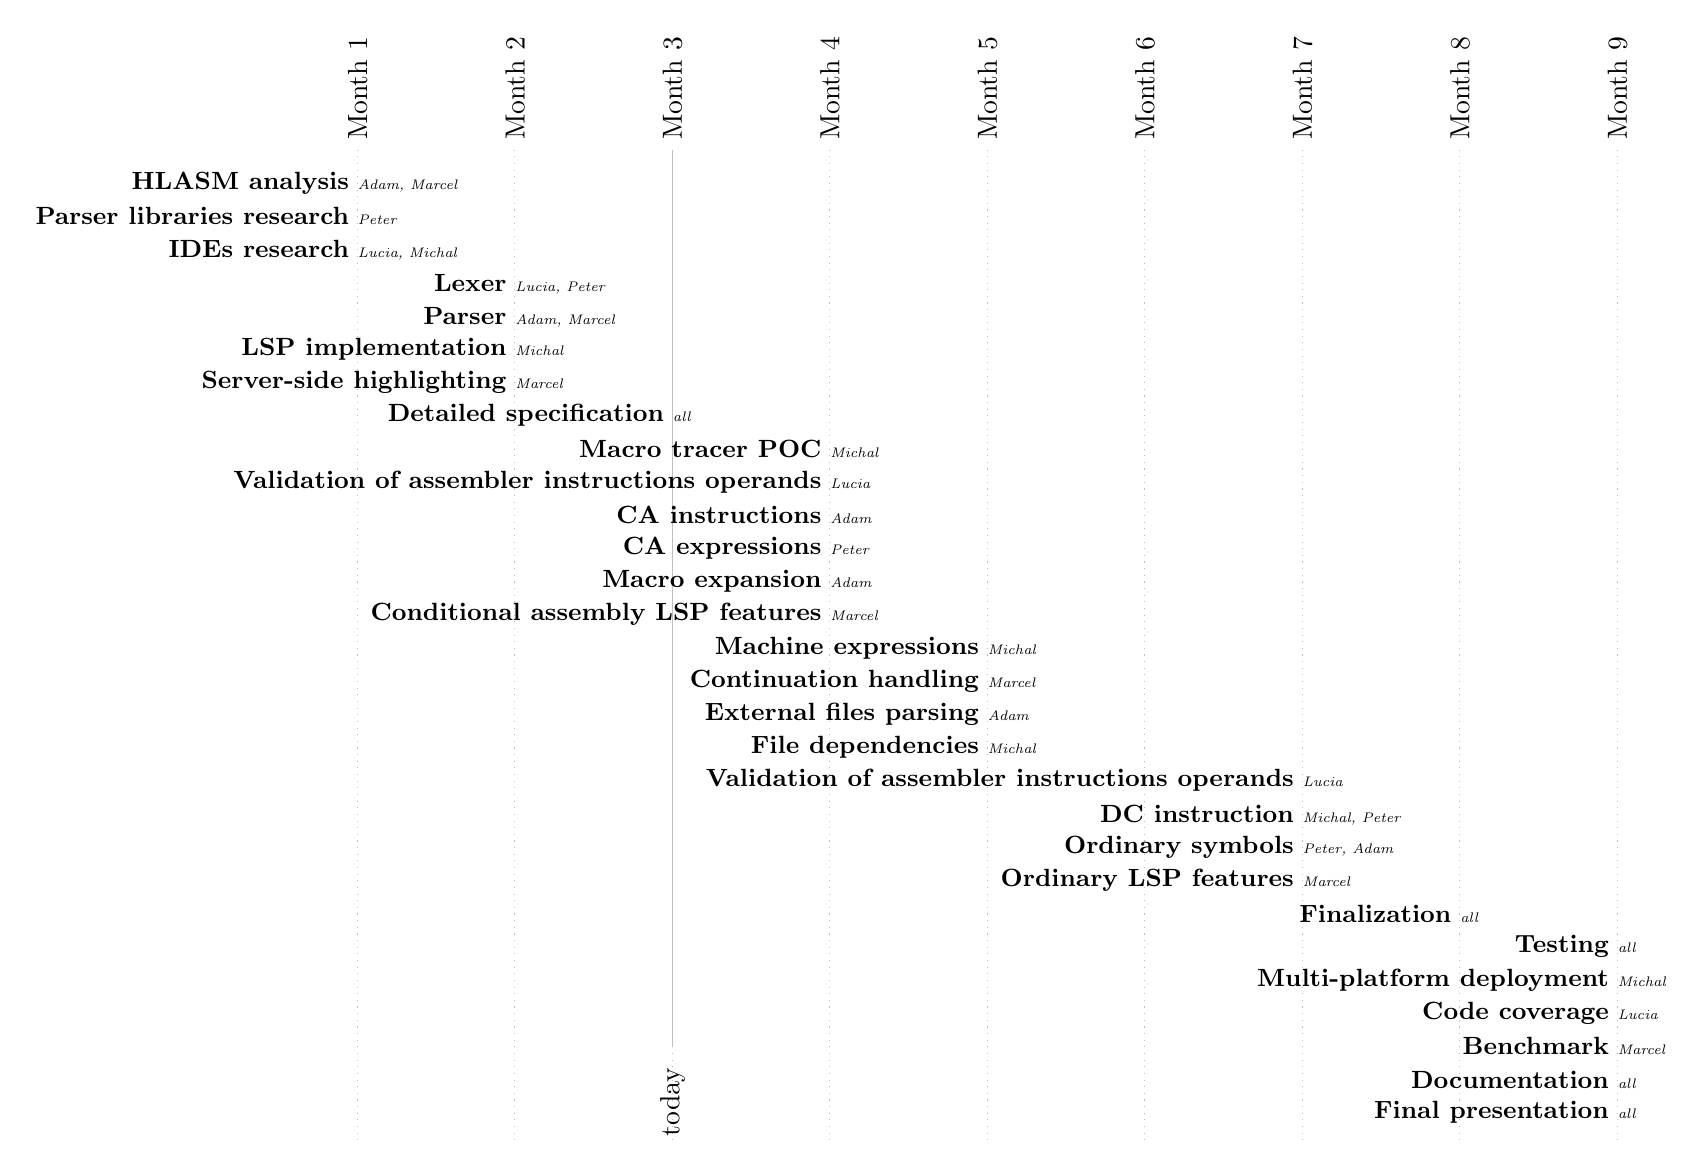
\begin{tikzpicture}
		\foreach \wp in {1,...,30} {
			\coordinate (wp\wp) at (0,\wp * -1.2em);
		};
		\foreach \tim in {1,...,9} {
			\coordinate (t\tim) at (\tim * 2cm,0);
			\node[month] at (t\tim) {Month \tim};
			\draw[dotted, thin, draw=black!25] (t\tim) to (t\tim |- wp30); %sync with previous
		};
		
		
		\draw[draw=black!25] (t3) to (t3 |- wp27); %sync with previous
		\node[month] at (t3|-wp30) {today};
		
		\ganttitem{ider}{t1|-wp3}{IDEs research}{Lucia, Michal};
		\ganttitem{pare}{t1|-wp2}{Parser libraries research}{Peter};
		\ganttitem{hlas}{t1|-wp1}{HLASM analysis}{Adam, Marcel};
		
		\ganttitem{lex}{t2|-wp4}{Lexer}{Lucia, Peter};
		\ganttitem{lex}{t2|-wp5}{Parser}{Adam, Marcel};
		\ganttitem{lsppoc}{t2|-wp6}{LSP implementation}{Michal}
		\ganttitem{vspoc}{t2|-wp7}{Server-side highlighting}{Marcel}

		
		\ganttitem{lex}{t3|-wp8}{Detailed specification}{all};
		
		
		\ganttitem{vspoc}{t4|-wp9}{Macro tracer POC}{Michal}
		\ganttitem{lex}{t4|-wp10}{Validation of assembler instructions operands}{Lucia};
		\ganttitem{lex}{t4|-wp11}{CA instructions}{Adam};
		\ganttitem{lex}{t4|-wp12}{CA expressions}{Peter};
		\ganttitem{lex}{t4|-wp13}{Macro expansion}{Adam};
		\ganttitem{lex}{t4|-wp14}{Conditional assembly LSP features}{Marcel};
		
		
		\ganttitem{lex}{t5|-wp15}{Machine expressions}{Michal};
		\ganttitem{lex}{t5|-wp16}{Continuation handling}{Marcel};
		\ganttitem{lex}{t5|-wp17}{External files parsing}{Adam};
		\ganttitem{lex}{t5|-wp18}{File dependencies}{Michal};
		
		
		\ganttitem{lex}{t7|-wp19}{Validation of assembler instructions operands}{Lucia};
		\ganttitem{lex}{t7|-wp20}{DC instruction}{Michal, Peter};
		\ganttitem{lex}{t7|-wp21}{Ordinary symbols}{Peter, Adam};
		\ganttitem{lex}{t7|-wp22}{Ordinary LSP features}{Marcel};
		
		
		\ganttitem{lex}{t8|-wp23}{Finalization}{all};
		
		\ganttitem{lex}{t9|-wp24}{Testing}{all};
		\ganttitem{lex}{t9|-wp25}{Multi-platform deployment}{Michal};
		\ganttitem{lex}{t9|-wp26}{Code coverage}{Lucia};
		\ganttitem{lex}{t9|-wp27}{Benchmark}{Marcel};
		
		\ganttitem{lex}{t9|-wp28}{Documentation}{all};
		\ganttitem{lex}{t9|-wp29}{Final presentation}{all};
		
		
		\end{tikzpicture}
		\caption{Work packages overview}
		\label{fig:gantt-pokus}
	\end{figure}
\end{landscape}











\iffalse

\bms
\itemm Research and analysis \deadline{2}{2}

\small The output of this milestone should be deeper knowledge and understanding of HLASM language, selection of parser library and target IDE.
HLASM is complicated language, hence the choice of right parser library is vital for further development. Also important is to choose IDE in witch would be the language support integrated.

\bwp
\itemwp HLASM language analysis \people{Adam, Marcel}
\tiny study and analysis of HLASM documentation, available code and discussion with HLASM users

\itemwp Parser libraries research \people{Peter}
\tiny research and comparison of contemporary lexical and parser libraries (Bison, ANTLR, ...) 

\itemwp IDEs research \people{Michal, Lucia}
\tiny research of available IDEs to which would be the HLASM language support integrated
\eenum


\itemm Parser prototype \deadline{3}{2}

\small With knowledge and selected tools from previous milestone, this milestone should output first prototype of parser.

\bwp
\itemwp Lexer \people{Lucia, Peter}
\itemwp Parser \people{Adam, Marcel}
\eenum


\itemm IDE integration prototype \deadline{3}{1}

\small In this milestone should be accomplished integration of the parser to the selected IDE.

\bwp
\itemwp LSP POC \people{Michal}
\tiny proof of concept of the Language Server Protocol (LSP) implementation (see chapter \hyperref[arch]{Architecture})

\itemwp VS Code client POC \people{Michal}
\tiny proof of concept of the \hyperref[arch:client]{VS Code client}

\itemwp Debugger POC \people{Michal}
\tiny proof of concept of the Debug Adapter Protocol (see \ref{arch:macro})
\eenum





\itemm \label{milestone_preview} Preview \deadline{4}{2}

\small Output of this milestone is working demo and its presentation in Broadcom. To accomplish this, several essential WPs must be done.

\bwp
\itemwp Client semantic highlighting \people{Marcel}
\tiny implementation of semantic highlighting in the IDE

\itemwp Assembler checker \people{Lucia}
\tiny validation of assembler instruction operands

\itemwp Conditional assembly instructions \people{Adam}
\tiny processing of conditional assembly instructions inside the Analyzer

\itemwp Conditional assembly expressions \people{Peter}
\tiny evaluation of conditional assembly expression 

\itemwp Macro expansion \people{Adam}
\tiny processing of macros (expansion)

\itemwp Conditional assembly LSP features \people{Marcel}
\tiny Hover, Go to definition and Find all references for variable symbols


\eenum




\itemm Detailed specification \deadline{6}{1}
\bwp
\itemwp Detailed specification \people{all}
\eenum


\itemm Features \deadline{7}{4}

\small Addition of other important features.

\bwp

\itemwp Machine expressions \people{Michal}
\tiny expressions that are used in assembler and machine instructions

\itemwp Machine instruction checker \people{Lucia}
\tiny validation of machine instruction operands

\itemwp DC instruction \people{Michal, Peter}
\tiny parsing, validation and length of data definition operand

\itemwp Copy instruction \people{Adam}
\tiny external files include

\itemwp Client-server continuation handling \people{Marcel}
\tiny implementation of support for continuation (see \cref{Continuation})

\itemwp Diagnostics \people{Lucia}
\tiny errors and warnings reporting polishing

\itemwp Ordinary LSP features \people{Marcel}
\tiny implementation of support for ordinary symbols

\itemwp Ordinary symbols \people{Adam, Peter}
\tiny ordinary assembly implementation
\eenum

\itemm Finalization \deadline{8}{1}

\small After this milestone should be all components finalized. 

\bwp
\itemwp Finalization \people{all}
\eenum

\itemm Feature testing \deadline{9}{2}

\small Goal of this milestone is to test, polish and benchmark all code from previous milestones.

\bwp
\itemwp Testing \people{all}

\itemwp Multiplatform deployment \people{Michal}
\tiny deployment on platforms Windows, Linux and Mac OS

\itemwp Code coverage \people{Lucia}

\itemwp Benchmarking \people{Marcel}
\eenum

\itemm Documentation \deadline{9}{1}

\small Goal is to assembly a complete documentation for whole work.

\bwp
\itemwp Documentation \people{all}
\eenum

\itemm Final presentation \deadline{9}{0}
\bwp
\itemwp Final presentation \people{all}
\eenum
\eenum



\newgeometry{a4paper,left=1in,right=1in,top=1in,bottom=1in,nohead}

\begin{landscape}
	\begin{figure}
		\centering
		\begin{ganttchart}[vgrid={draw=none, dotted}, x unit = 1.2cm]{1}{12}
		
		\gantttitlelist{"1. month", "2. month", "3. month"}{4} \\
		\gantttitlelist{1,...,12}{1} \\
		
		\ganttbar{HLASM language analysis (A \& Ma)}{1}{8} \\
		\ganttbar{Parser libraries research (P)}{1}{4}\\
		\ganttbar{IDEs research (L \& Mi)}{1}{4}\\
		
		\ganttbar{LSP POC (Mi)}{5}{8} \\
		\ganttbar{VSCode client POC(Mi)}{5}{8}\\
		\ganttbar{Lexer (L \& P)}{5}{10}\\
		\ganttbar{Parser (A \& Ma)}{5}{12}\\
		
		\ganttbar{Client semantic highlighting (Ma)}{9}{12}\\
		\ganttbar{Assembler checker (L)}{9}{12}\\
		\ganttbar{Debugger POC (Mi)}{9}{12}\\
		\ganttbar{Conditional assembly instructions (A)}{9}{12}\\
		\ganttbar{Conditional assembly expressions (P) $\rightarrow$}{11}{12}\\
		
		\ganttvrule[vrule offset=0.8]{today}{12}
		
		\end{ganttchart}
    \caption{Tasks for months 1 -- 3}
	\label{fig:gantt1}
	\end{figure}
\end{landscape}


\begin{landscape}
	\begin{figure}
		\centering
		\begin{ganttchart}[vgrid={draw=none, dotted}, x unit = 1.2cm]{1}{12}
			
			\gantttitlelist{"4. month", "5. month", "6. month"}{4} \\
			\gantttitlelist{13,...,24}{1} \\
			\ganttbar{$\rightarrow$ Conditional assembly expressions (P)}{1}{2}\\
			\ganttbar{Macro expansion (A)}{1}{4}\\
			\ganttbar{Conditional assembly LSP features (Ma)}{1}{4}\\
			\ganttbar{Machine expressions (Mi)}{1}{4}\\
			
			\ganttmilestone{Demo presentation}{4}\\
			
			\ganttbar{Machine instruction checker (L)}{1}{12}\\
			\ganttbar{DC instruction (Mi \& P)}{3}{12}\\
			
			\ganttbar{Copy instruction (A)}{5}{8}\\
			\ganttbar{Client-server continuation handling (Ma)}{5}{8}\\
			
			\ganttbar{Diagnostics (L)}{9}{12} \\
			\ganttbar{Ordinary LSP features (Ma)}{9}{12}\\
			\ganttbar{Ordinary symbols (A \& P) $\rightarrow$}{9}{12}
			
			
			
		\end{ganttchart}
		\caption{Tasks for months 4 -- 6}
		\label{fig:gantt2}
	\end{figure}
\end{landscape}

\begin{landscape}
	\begin{figure}
		\centering
		\begin{ganttchart}[vgrid={draw=none, dotted}, x unit = 1.2cm]{1}{12}
			
			\gantttitlelist{"7. month", "8. month", "9. month"}{4} \\
			\gantttitlelist{25,...,36}{1} \\
			
			
			\ganttbar{$\rightarrow$ Ordinary symbols (A \& P)}{1}{4}\\
			\ganttbar{Multiplatform deployment (Mi)}{1}{4}\\
			\ganttbar{Benchmarking (Ma)}{1}{4}\\
			\ganttbar{Code coverage (L)}{1}{8}\\
			
			\ganttbar{Testing (all)}{5}{12}\\
			
			\ganttbar{Documentation (all)}{9}{12}\\
		
			
			\ganttvrule[vrule offset=0.2]{today}{1}
			
		\end{ganttchart}
		\caption{Tasks for months 7 -- 9}
		\label{fig:gantt3}
	\end{figure}
\end{landscape}

\restoregeometry
\fi



